\section{Đánh đổi riêng tư, chất lượng và tài nguyên truy hồi}
\label{sec:coverage-frontier-experiment}

\subsection{Thiết kế phép so sánh}

Phép thử xét bốn bộ chọn: BR-làn theo hình học; phủ trung bình với prior đều trên ô công khai; cùng hàm mục tiêu nhưng cho phép thay điểm; và phủ cân bằng có cắt ngưỡng loại dịch vụ. Mỗi bộ chọn chạy với $B\in\{0{,}12;0{,}24;0{,}48\}\,\mathrm{m}^{-1}$, $K=5$, $H=12$ và $\theta=200$ m. Tại cùng $B$, các phương pháp dùng cùng dữ liệu thật và cùng dãy neo bảo vệ. Hai biến thể mới không thay cơ chế neo, lịch gửi hoặc số lượng điểm công bố.

Dữ liệu gồm chín ca S1--S3 từ các nhóm đã được xem trong quá trình phát triển. Hai nhóm 101--102 dùng để học, 103--104 dùng để chọn, 201--204 dùng để đối chiếu phát triển, với ba lần lặp ngẫu nhiên theo từng bản ghi. Thêm 256 cửa sổ từ 64 nhóm SUMO phụ trợ chỉ phục vụ huấn luyện đối thủ. Tập 16 nhóm phụ trợ giữ lại không được sử dụng trong vòng này. Không có nhóm xác nhận mới và không mở rộng tuyên bố bảo vệ sang S4--S8.

Mỗi cặp phương pháp--ngân sách có bộ đối thủ riêng nhưng cùng lượng dữ liệu học: 360 quan sát lõi và 2.873 quan sát phụ trợ, tổng 3.233 quan sát. Giữ cả các bộ suy luận trên dữ liệu lõi, trên dữ liệu mở rộng, hai bộ hồi quy cây và các đối thủ trực tiếp từ tập/chuỗi điểm công bố. Đối thủ MAE và Hit được chọn riêng cho từng ca trên validation trước khi chấm phát triển. Cực trị trong toàn bộ bộ đối thủ được báo cáo thêm để chỉ ra hạn chế của cách chọn, không thay thế kết quả đã khoá.

Hai mức phản hồi $L=5$ và $L=10$ được chấm trên cùng tọa độ công bố; top-5 tham chiếu không thay đổi. Tất cả phương pháp đều được cấp cả hai mức. Các kết quả trong bảng lấy trung bình đều qua chín ca; mỗi ca lấy trung bình các nhóm và lần lặp, mỗi bản ghi lấy trung bình các truy vấn loại--thời điểm có đáp án tham chiếu. Các loại không có tham chiếu được đếm riêng, không coi là trả lời đúng. Thời gian sinh đo tuần tự riêng trên ba bản ghi validation thuộc một nhóm, tách khỏi thời gian chạy thí nghiệm đồng thời.

\subsection{Kết quả theo ngân sách và độ sâu phản hồi}

\begin{table}[htbp]
\centering\small
\setlength{\tabcolsep}{3pt}
\caption{Biên thực nghiệm với phản hồi top-5; đáp án tham chiếu luôn top-5. Recall và Hit tính theo phần trăm; byte là danh sách ID mỗi sự kiện. Hit chọn trên validation khác cực trị thăm dò.}\label{tab:coverage-frontier-5}
\begin{tabular}{rlrrrrr}
\toprule
$B$ & Bộ chọn & Recall & Ca thấp & Hit chọn & Hit cực trị & Byte\\\midrule
0.12 & BR-làn & 80.03 & 71.67 & 2.85 & 7.04 & 2737\\
0.12 & Phủ trung bình & 87.69 & 83.81 & 1.34 & 6.59 & 2737\\
0.12 & Phủ + thay điểm & 88.40 & 84.68 & 0.93 & 9.29 & 2737\\
0.12 & Phủ cân bằng & 88.10 & 83.79 & 0.00 & 9.59 & 2738\\
0.24 & BR-làn & 87.48 & 84.01 & 8.65 & 17.05 & 2728\\
0.24 & Phủ trung bình & 92.35 & 86.01 & 3.76 & 16.23 & 2738\\
0.24 & Phủ + thay điểm & 92.93 & 86.36 & 5.99 & 16.17 & 2738\\
0.24 & Phủ cân bằng & 91.99 & 86.94 & 2.66 & 16.61 & 2738\\
0.48 & BR-làn & 91.37 & 85.43 & 17.73 & 26.00 & 2726\\
0.48 & Phủ trung bình & 94.22 & 85.65 & 5.42 & 19.87 & 2738\\
0.48 & Phủ + thay điểm & 94.95 & 87.42 & 4.02 & 20.42 & 2737\\
0.48 & Phủ cân bằng & 93.98 & 87.82 & 3.41 & 18.89 & 2736\\
\bottomrule
\end{tabular}
\end{table}

\begin{table}[htbp]
\centering\small
\setlength{\tabcolsep}{3pt}
\caption{Biên thực nghiệm với phản hồi top-10; đáp án tham chiếu luôn top-5. Recall và Hit tính theo phần trăm; byte là danh sách ID mỗi sự kiện. Hit chọn trên validation khác cực trị thăm dò.}\label{tab:coverage-frontier-10}
\begin{tabular}{rlrrrrr}
\toprule
$B$ & Bộ chọn & Recall & Ca thấp & Hit chọn & Hit cực trị & Byte\\\midrule
0.12 & BR-làn & 86.41 & 81.38 & 2.85 & 7.04 & 4511\\
0.12 & Phủ trung bình & 92.28 & 88.50 & 1.34 & 6.59 & 4512\\
0.12 & Phủ + thay điểm & 92.36 & 89.04 & 0.93 & 9.29 & 4511\\
0.12 & Phủ cân bằng & 92.13 & 88.36 & 0.00 & 9.59 & 4512\\
0.24 & BR-làn & 92.85 & 90.85 & 8.65 & 17.05 & 4498\\
0.24 & Phủ trung bình & 96.12 & 92.31 & 3.76 & 16.23 & 4513\\
0.24 & Phủ + thay điểm & 96.38 & 92.44 & 5.99 & 16.17 & 4513\\
0.24 & Phủ cân bằng & 96.01 & 93.26 & 2.66 & 16.61 & 4510\\
0.48 & BR-làn & 95.48 & 92.53 & 17.73 & 26.00 & 4495\\
0.48 & Phủ trung bình & 97.12 & 92.04 & 5.42 & 19.87 & 4513\\
0.48 & Phủ + thay điểm & 97.65 & 94.59 & 4.02 & 20.42 & 4513\\
0.48 & Phủ cân bằng & 96.87 & 93.43 & 3.41 & 18.89 & 4506\\
\bottomrule
\end{tabular}
\end{table}

\begin{table}[htbp]
\centering\small
\setlength{\tabcolsep}{3pt}
\caption{Sai số suy luận (m) và thời gian sinh (ms). Thời gian đo tuần tự riêng trên ba bản ghi validation, không phải tốc độ thiết bị di động; MAE không đổi khi chỉ tăng độ sâu phản hồi.}\label{tab:coverage-frontier-timing}
\begin{tabular}{rlrrrr}
\toprule
$B$ & Bộ chọn & MAE chọn & MAE cực trị & Bước TB & Bước p95\\\midrule
0.12 & BR-làn & 1346.5 & 736.7 & 6.6 & 29.8\\
0.12 & Phủ trung bình & 1469.5 & 805.0 & 18.8 & 85.8\\
0.12 & Phủ + thay điểm & 1505.3 & 810.2 & 24.0 & 130.5\\
0.12 & Phủ cân bằng & 1555.8 & 792.0 & 28.0 & 161.0\\
0.24 & BR-làn & 747.9 & 426.1 & 6.5 & 30.0\\
0.24 & Phủ trung bình & 1110.1 & 503.8 & 18.8 & 85.8\\
0.24 & Phủ + thay điểm & 1086.0 & 526.4 & 24.0 & 150.7\\
0.24 & Phủ cân bằng & 1216.0 & 515.0 & 28.9 & 171.6\\
0.48 & BR-làn & 365.7 & 283.3 & 6.2 & 29.7\\
0.48 & Phủ trung bình & 919.7 & 414.1 & 18.2 & 83.5\\
0.48 & Phủ + thay điểm & 865.5 & 434.1 & 18.5 & 103.0\\
0.48 & Phủ cân bằng & 1037.1 & 457.7 & 29.9 & 173.0\\
\bottomrule
\end{tabular}
\end{table}

\begin{table}[htbp]
\centering\small
\setlength{\tabcolsep}{3pt}
\caption{Cấu hình chọn trước khi chấm phát triển. Điều kiện là Recall thấp nhất theo ca đạt 90\% trên validation; không có ứng viên thì không chọn phương án thay thế. Hai cột cuối là Recall của ca thấp nhất (\%).}\label{tab:coverage-frontier-selection}
\begin{tabular}{rrlrr}
\toprule
$B$ & $L$ & Chọn trên validation & Validation & Phát triển\\\midrule
0.12 & 5 & Không có & --- & ---\\
0.12 & 10 & Không có & --- & ---\\
0.24 & 5 & Không có & --- & ---\\
0.24 & 10 & Phủ + thay điểm & 91.37 & 92.44\\
0.48 & 5 & Phủ + thay điểm & 91.61 & 87.42\\
0.48 & 10 & Phủ + thay điểm & 93.06 & 94.59\\
\bottomrule
\end{tabular}
\end{table}


\clearpage
\begin{figure}[H]
\centering
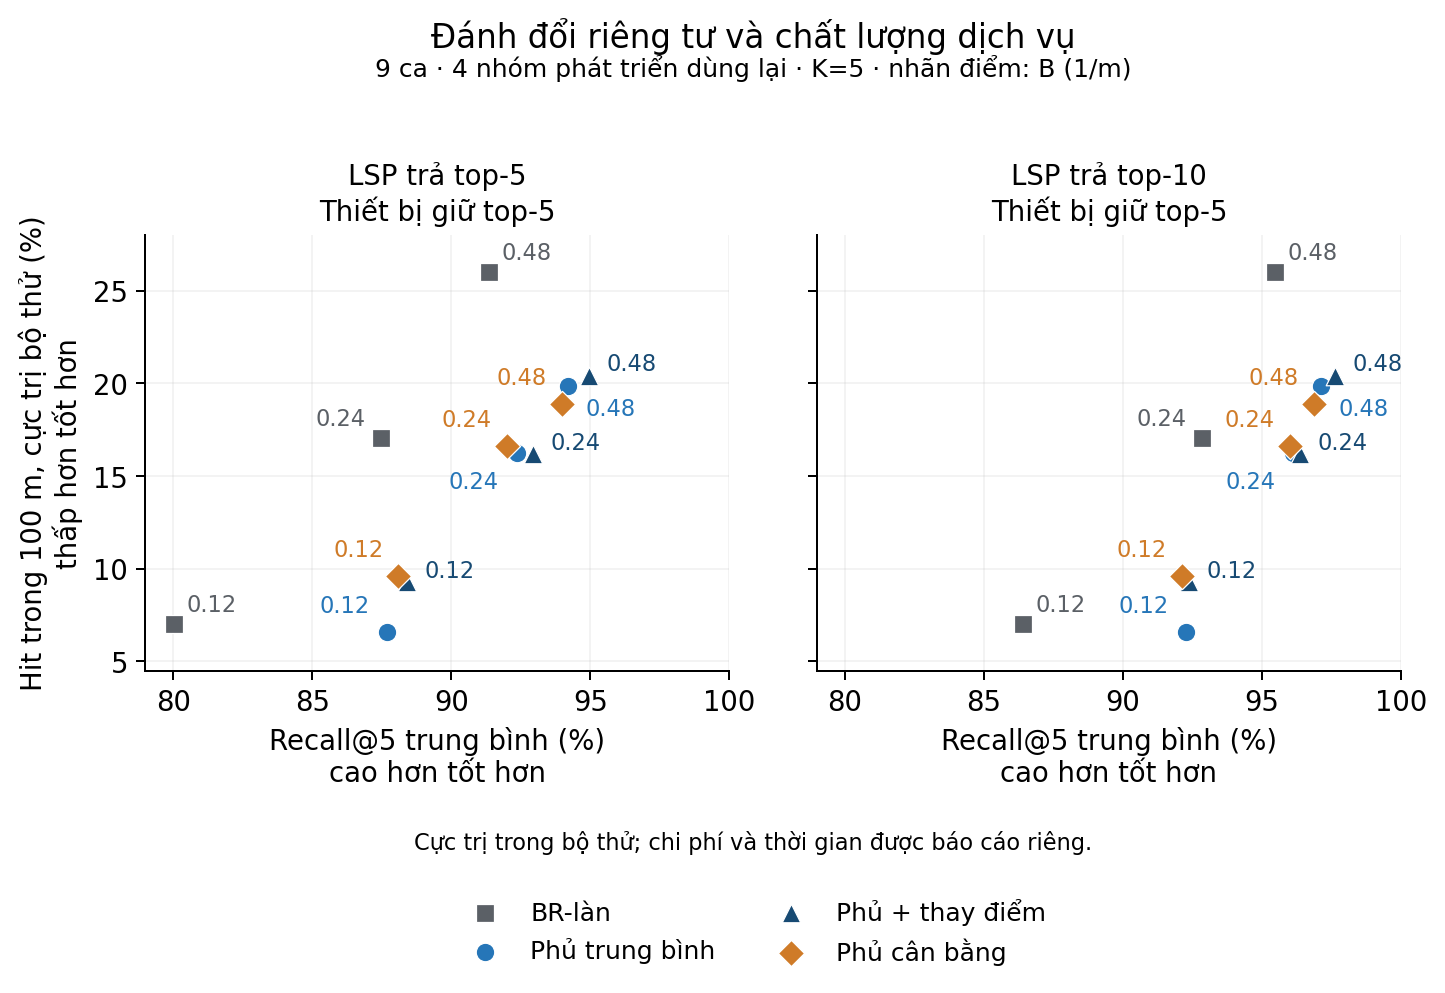
\includegraphics[width=\textwidth]{../artifacts/benchmarks/coverage_frontier/frontier.png}
\caption{Recall@5 và Hit cực trị trong bộ đối thủ đã thử. Mỗi điểm là một cặp bộ chọn--ngân sách, cùng bốn nhóm phát triển đã dùng lại. Biểu đồ không thể hiện toàn bộ chi phí hay độ bất định và không được đọc như bảng xếp hạng SOTA.}
\label{fig:coverage-frontier}
\end{figure}

\subsection{Phân biệt cải thiện thuật toán và tăng tài nguyên}

Ở cùng $B=0{,}24$, $K=5$ và $L=5$, thêm bước thay điểm nâng Recall trung bình từ 92,35\% lên 92,93\%; ca thấp nhất chỉ tăng từ 86,01\% lên 86,36\%, vẫn chưa đạt yêu cầu dịch vụ. Mức tăng trung bình xuất hiện ở cả bốn nhóm phát triển, trong khoảng 0,04--1,12 điểm phần trăm. Với hai ngân sách còn lại, bước thay điểm cũng tăng Recall trung bình ở $L=5$ trên cả bốn nhóm. Đây là bằng chứng thuận lợi cho bước tối ưu tập truy vấn, nhưng quy mô nhóm nhỏ và đã dùng lại chưa cho phép kết luận tổng quát.

Khi giữ bộ chọn phủ trung bình và chỉ tăng phản hồi từ top-5 lên top-10 tại $B=0{,}24$, Recall tăng từ 92,35\% lên 96,12\%. Thay bộ chọn bằng bản có thay điểm tại \emph{cùng} top-10 chỉ tăng tiếp lên 96,38\%, với ca thấp nhất 92,44\%. Như vậy, trong mức tăng tổng cộng khoảng 4,03 điểm phần trăm so với cấu hình cũ, khoảng 3,78 điểm đến từ độ sâu phản hồi và 0,26 điểm từ thay bộ chọn ở cùng độ sâu. Không quy toàn bộ lợi ích đó cho thuật toán mới. Ở $L=10$, một nhóm tại $B=0{,}24$ còn giảm 0,14 điểm phần trăm khi thêm bước thay; lợi ích không đồng đều trên mọi nhóm và mức tài nguyên.

Biến thể phủ cân bằng không trở thành lựa chọn mặc định. Tại $B=0{,}24$, Recall ở $L=5$ là 91,99\%, thấp hơn bản phủ trung bình; ba trong bốn nhóm suy giảm. Nó nâng ca thấp nhất nhưng không đồng thời nâng chất lượng trung bình, và không đạt ngưỡng chọn trên validation ở cả hai độ sâu. Tại $B=0{,}48$, nó cũng giảm Recall trung bình so với phủ trung bình. Chuẩn hoá và cắt ngưỡng một hàm gần đúng chưa đủ để bảo vệ ca khó; kết quả âm này không được bỏ khỏi phép so sánh.

Với bộ chọn có thay điểm tại $B=0{,}24$, tăng $L$ làm số mục phản hồi trung bình tăng từ 120 lên 200 mỗi sự kiện; byte danh sách ID tăng từ khoảng 2.738 lên 4.513, tức gần 65\%, dù số yêu cầu vẫn là 30. Số mục thực nhận nhỏ hơn giới hạn $6KL$ do một số loại có ít POI khả dụng. Phép đo tuần tự riêng cho thấy thời gian mỗi bước tăng từ trung bình 18,8 ms của phủ tham lam lên 24,0 ms khi thêm thay điểm; p95 tăng từ 85,8 lên 150,7 ms. Mỗi cấu hình chỉ có 20 bước từ ba bản ghi trong phép đo này, nên chưa đại diện độ trễ trên điện thoại hay tải dịch vụ thật.

\subsection{Riêng tư và khả năng chuyển giao của phép chọn}

Tăng chất lượng không kéo theo tăng riêng tư. Tại $B=0{,}24$, thêm thay điểm làm Hit của đối thủ chọn trên validation tăng từ 3,76\% lên 5,99\%, còn Hit cực trị trong bộ đã thử gần như không đổi: 16,23\% xuống 16,17\%. Chưa có cơ sở gọi đây là cải thiện riêng tư. Tại $B=0{,}48$, Hit chọn giảm nhưng Hit cực trị lại tăng, tiếp tục cho thấy cần đọc cả hai cột.

Một phản ví dụ rõ là phủ cân bằng tại $B=0{,}12$: Hit chọn bằng 0\% nhưng cực trị phát triển là 9,59\%. Con số 0 không có nghĩa đối thủ không thể định vị; nó cho thấy quyết định chọn trên tập nhỏ không chuyển giao tốt. Cực trị cũng chỉ phản ánh bộ tấn công hữu hạn đã thử, không phải đối thủ tối ưu. Các chặn Geo-I ở ba mức $B$ vẫn lỏng tại khoảng cách 100 m; không xếp hạng ngân sách bằng riêng lỗi thực nghiệm của bộ đối thủ này.

Quy tắc chọn ghi nhận không có phương pháp khả thi ở $B=0{,}12$ cho cả hai độ sâu, và ở $B=0{,}24$, $L=5$. Với $B=0{,}24$, $L=10$, bản phủ có thay điểm là ứng viên được chọn, đạt ca thấp nhất 91,37\% trên validation và 92,44\% trên phát triển. Bản phủ trung bình ở cùng điều kiện chỉ đạt 89,96\% trên validation, nên không được làm tròn thành đạt 90\% dù kết quả phát triển tốt hơn ngưỡng.

Ở $B=0{,}48$, bản có thay điểm được chọn tại cả hai độ sâu. Tuy nhiên, tại $L=5$, ca thấp nhất giảm từ 91,61\% trên validation xuống 87,42\% trên phát triển; chỉ $L=10$ giữ được ngưỡng trong dữ liệu đã thử. Kết quả này phân biệt \emph{được chọn} với \emph{giữ được chất lượng sau lựa chọn}. Cấu hình $B=0{,}24$, $L=10$ là ứng viên hợp lý cho vòng xác nhận riêng tiếp theo, không phải mô hình đã xác nhận hoặc quyết định triển khai mặc định.

\subsection{Ý nghĩa đối với hướng nghiên cứu}

Thực nghiệm ủng hộ hướng cải thiện bộ chọn tập truy vấn và thiết kế dịch vụ phối hợp tại thiết bị, nhưng chưa ủng hộ ưu thế riêng tư của bước thay điểm hay tính bền vững của cắt ngưỡng. Đóng góp có thể kiểm chứng ở giai đoạn này là đặc tả rõ quyết định nhân quả, miền chuyển động khả thi, tác vụ truy hồi cố định và chi phí; sau đó đo riêng tác động của từng thành phần. Vòng tiếp theo cần tập chọn đa dạng hơn và nhóm xác nhận mới, cùng kiểm tra đối thủ mạnh hơn, trước khi quy kết thành ưu thế thuật toán trong bài báo.


\subsection{Giới hạn của đóng góp}

Một bước thay điểm tăng hàm mục tiêu gần đúng chưa bảo đảm tăng Recall thật: prior có thể lệch, ngưỡng có thể ngừng thưởng quá sớm và vị trí chọn hiện tại quyết định miền tới được về sau. Hai thao tác chuẩn hoá loại dịch vụ và cắt ngưỡng đi cùng nhau trong biến thể cân bằng; cần phân rã riêng nếu quy kết lợi ích cho từng thao tác. Cả hai phép tối ưu là thành phần kế thừa, không phải cơ sở đủ để khẳng định tính mới.

Biên thực nghiệm được xét trong từng $B$, với chất lượng, rủi ro suy luận và byte phản hồi; thời gian được bổ sung như phép đo cục bộ riêng. Không tuyên bố một ngân sách bảo vệ lỏng hơn tốt hơn chỉ dựa vào lỗi của đối thủ đã thử. Lưới này là phân tích thành phần trên cùng giao diện dummy-only. Đối chứng khác giao diện và mô hình gốc vẫn cần tái lập/điều chỉnh có giải thích trước khi đưa ra kết luận vượt SOTA.
